\documentclass[aspectratio=169,11pt]{beamer}
\usepackage[T1]{fontenc}
\usepackage{lmodern,amsmath,amssymb,mathtools,bm,booktabs,array,graphicx,tikz}
\usetikzlibrary{arrows.meta,positioning,calc,decorations.pathreplacing,patterns}
\definecolor{ink}{HTML}{17344D}\definecolor{accent}{HTML}{087E8B}\definecolor{pale}{HTML}{EDF5F5}\definecolor{gold}{HTML}{AD6B19}
\providecommand{\dd}{\,\mathrm{d}}\providecommand{\R}{\mathbb{R}}
\providecommand{\E}{\mathbb{E}}\providecommand{\Var}{\operatorname{Var}}
\providecommand{\Cov}{\operatorname{Cov}}\providecommand{\diag}{\operatorname{diag}}
\providecommand{\norm}[1]{\left\lVert#1\right\rVert}
\providecommand{\abs}[1]{\left|#1\right|}
\usefonttheme{professionalfonts}
\setbeamercolor{normal text}{fg=black,bg=white}
\setbeamercolor{frametitle}{fg=ink,bg=white}
\setbeamercolor{title}{fg=ink}\setbeamercolor{structure}{fg=accent}
\setbeamercolor{block title}{fg=ink,bg=pale}\setbeamercolor{block body}{fg=black,bg=pale!40}
\setbeamercolor{alerted text}{fg=accent}
\setbeamerfont{frametitle}{size=\Large,series=\bfseries}
\setbeamerfont{title}{size=\LARGE,series=\bfseries}
\setbeamertemplate{navigation symbols}{}
\setbeamersize{text margin left=.7cm,text margin right=.7cm}
\setbeamertemplate{frametitle}{\vspace{.18cm}\insertframetitle\par\vspace{.1cm}{\color{accent}\hrule height .6pt}\vspace{.12cm}}
\newcommand{\notestarget}{notes.pdf}\newcommand{\noteslabel}{Notes}
\setbeamertemplate{footline}{\hspace{.7cm}\color{ink}\scriptsize Mathematical Cardiology\quad\href{\notestarget}{\noteslabel}\hfill\insertframenumber\,/\,\inserttotalframenumber\hspace{.7cm}\vspace{.18cm}}
\setbeamercovered{invisible}
\hypersetup{pdfauthor={Zan Ahmad},pdftitle={Local image filters and learned classification},pdfpagemode=UseNone}
\begin{document}
\begin{frame}[plain]\vfill
{\small\color{accent} Mathematical Cardiology \quad Lecture 10}\par\medskip
{\raggedright\hyphenpenalty=10000\exhyphenpenalty=10000\LARGE\bfseries\color{ink} Local image filters and learned classification}\par\bigskip
Zan Ahmad\par\smallskip
{\small Fall 2023}\par\vfill\end{frame}
\renewcommand{\notestarget}{notes.pdf\#note-an-image-a-mask-and-a-label}
\begin{frame}[t,fragile,label=slide-specify-the-output]{Specify the output}
\[I\in\R^{16\times16}.\]
Classification returns one label: wide or tall.
\pause{}
Segmentation returns a label at each location.
A correct whole-image label does not establish a correct boundary.
\end{frame}
\renewcommand{\notestarget}{notes.pdf\#note-a-local-weighted-sum}
\begin{frame}[label=slide-a-fixed-directional-kernel-figure]{A fixed directional kernel}
\centering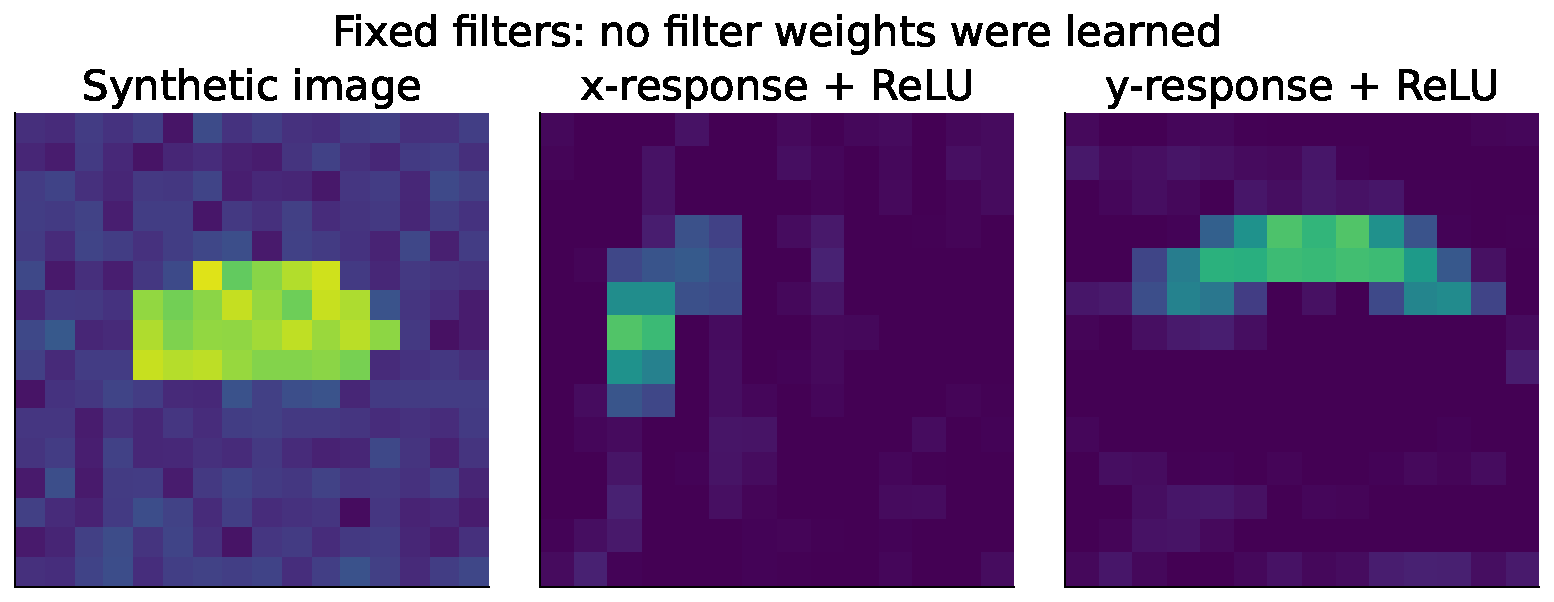
\includegraphics[width=.98\linewidth,height=.69\textheight,keepaspectratio]{image-filters.pdf}\end{frame}
\renewcommand{\notestarget}{notes.pdf\#note-a-local-weighted-sum}
\begin{frame}[t,fragile,label=slide-a-fixed-directional-kernel]{A fixed directional kernel}
\[K_x=\frac13\begin{pmatrix}-1&0&1\\-1&0&1\\-1&0&1\end{pmatrix},\qquad K_y=K_x^T.\]
\pause{}
Negative weights are on one side and positive weights on the other.
\end{frame}
\renewcommand{\notestarget}{notes.pdf\#note-a-local-weighted-sum}
\begin{frame}[t,fragile,label=slide-calculate-one-response]{Calculate one response}
For a patch with three identical rows $(0,0,1)$,
\[A^x=3\left[(-1)(0)/3+0(0)+(1)(1)/3\right]=1.\]
\pause{}
Rows $(1,0,0)$ give $-1$; a constant patch gives zero.
\end{frame}
\renewcommand{\notestarget}{notes.pdf\#note-a-local-weighted-sum}
\begin{frame}[t,fragile,label=slide-reuse-the-local-calculation]{Reuse the local calculation}
\[A^x_{ij}=\sum_{a=0}^2\sum_{b=0}^2(K_x)_{ab}I_{i+a,j+b}.\]
\pause{}
The same kernel is used at every valid window.
The code does not reverse the kernel: this is a sliding dot product.
\end{frame}
\renewcommand{\notestarget}{notes.pdf\#note-a-local-weighted-sum}
\begin{frame}[t,fragile,label=slide-count-the-valid-window-starts]{Count the valid window starts}
With size $N$, kernel width $k$, stride one and no padding,
\[N_{\rm out}=N-k+1.\]
\pause{}
\[16-3+1=14.\]
Each output map is $14\times14$.
\end{frame}
\renewcommand{\notestarget}{notes.pdf\#note-nonlinearity-averaging-and-information-loss}
\begin{frame}[t,fragile,label=slide-retain-only-positive-responses]{Retain only positive responses}
\[B^x_{ij}=\max(A^x_{ij},0).\]
\pause{}
ReLU preserves positive rises and discards negative responses.
For supplied intensities in $[0,1]$, $0\leq B^x_{ij}\leq1$.
\end{frame}
\renewcommand{\notestarget}{notes.pdf\#note-nonlinearity-averaging-and-information-loss}
\begin{frame}[t,fragile,label=slide-pool-the-maps-into-two-numbers]{Pool the maps into two numbers}
\[f_x=\frac1{196}\sum_{ij}B^x_{ij},\qquad
f_y=\frac1{196}\sum_{ij}B^y_{ij}.\]
\pause{}
The average keeps a response magnitude and loses its location.
\end{frame}
\renewcommand{\notestarget}{notes.pdf\#note-nonlinearity-averaging-and-information-loss}
\begin{frame}[t,fragile,label=slide-an-exact-transpose-check]{An exact transpose check}
The kernels satisfy $K_y=K_x^T$.
\pause{}
Transposing the image exchanges the pooled features:
\[\boxed{f(I^T)=(f_y(I),f_x(I))}.\]
A wide ellipse becomes tall relative to the axes.
\end{frame}
\renewcommand{\notestarget}{notes.pdf\#note-fitted-centers-and-learnable-convolutional-weights}
\begin{frame}[t,fragile,label=slide-fit-the-output-rule]{Fit the output rule}
From training images only,
\[c_k=\frac1{n_k}\sum_{i:y_i=k}f(I_i).\]
\pause{}
Predict the nearer center in squared Euclidean distance.
No feature-standardization fit is used in this pipeline.
\end{frame}
\renewcommand{\notestarget}{notes.pdf\#note-fitted-centers-and-learnable-convolutional-weights}
\begin{frame}[t,fragile,label=slide-weight-sharing-is-not-training]{Weight sharing is not training}
One $3\times3$ kernel has nine weights.
They are reused at $196$ locations.
\pause{}
Separate weights at each location would require
\[196\cdot9=1764\]
weights for one output map, before biases.
\end{frame}
\renewcommand{\notestarget}{notes.pdf\#note-fitted-centers-and-learnable-convolutional-weights}
\begin{frame}[t,fragile,label=slide-a-learned-convolution-would-update-the-kernels]{A learned convolution would update the kernels}
One possible extension has score
\[s_i=w^Tf_K(I_i)+b\]
and loss $\frac1n\sum_i(s_i-y_i)^2$.
\pause{}
Training would update selected parameters, including $K$.
The supplied filters remain fixed.
\end{frame}
\renewcommand{\notestarget}{notes.pdf\#note-evaluate-the-frozen-rule}
\begin{frame}[label=slide-the-held-out-image-counts-figure]{The held-out image counts}
\centering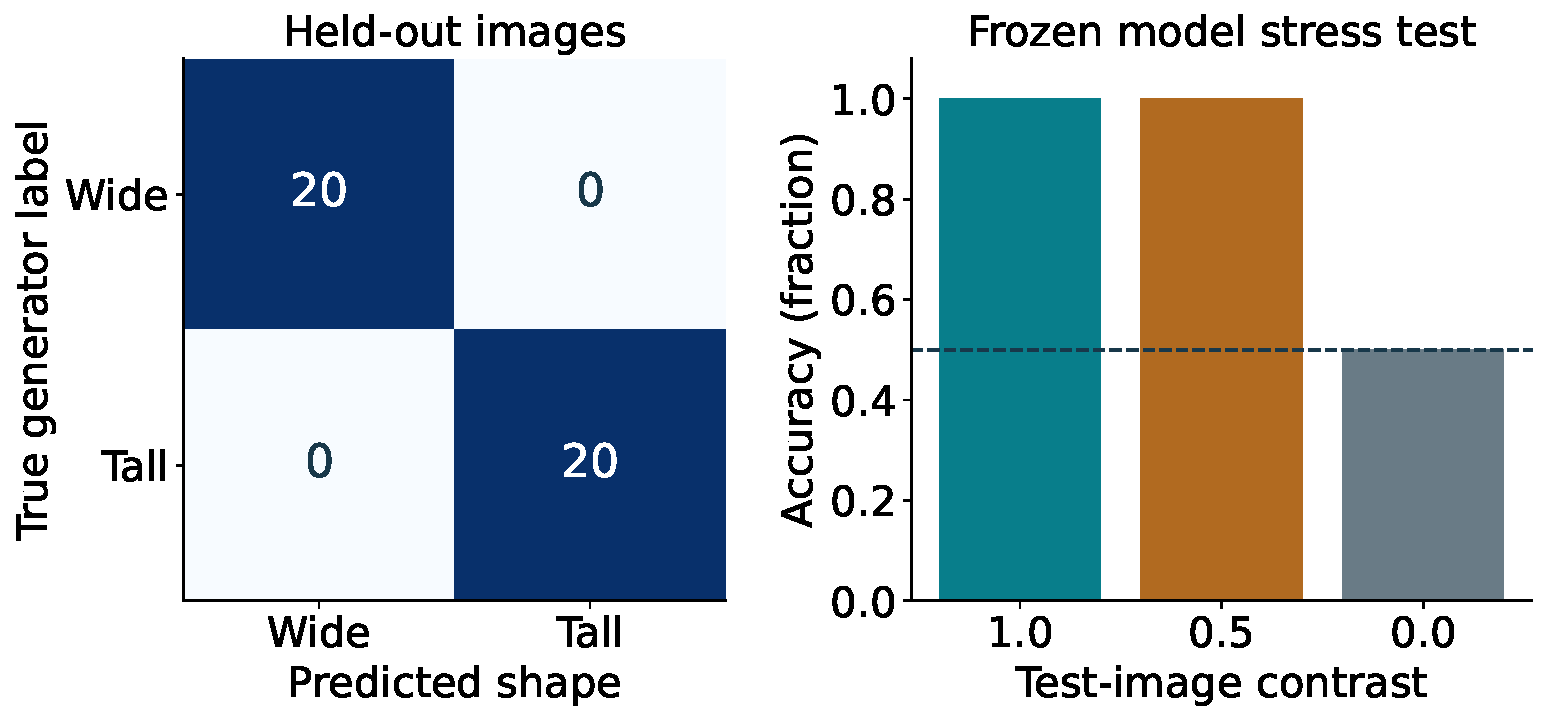
\includegraphics[width=.98\linewidth,height=.69\textheight,keepaspectratio]{image-evaluation.pdf}\end{frame}
\renewcommand{\notestarget}{notes.pdf\#note-evaluate-the-frozen-rule}
\begin{frame}[t,fragile,label=slide-the-held-out-image-counts]{The held-out image counts}
\[
\begin{array}{c|rr}
\text{true}\backslash\text{predicted}&\text{wide}&\text{tall}\\\hline
\text{wide}&20&0\\
\text{tall}&0&20
\end{array}
\]
\pause{}
Forty correct predictions on this synthetic test.
\end{frame}
\renewcommand{\notestarget}{notes.pdf\#note-contrast-target-transformations-and-a-defensible-conclusion}
\begin{frame}[t,fragile,label=slide-remove-the-signal-without-refitting]{Remove the signal without refitting}
\[
\begin{array}{c|ccc}
\text{contrast}&1&0.5&0\\\hline
\text{accuracy}&1&1&0.5
\end{array}
\]
\pause{}
At zero contrast the intended ellipse signal disappears.
Report all tested levels, not the most favorable one.
\end{frame}
\renewcommand{\notestarget}{notes.pdf\#note-contrast-target-transformations-and-a-defensible-conclusion}
\begin{frame}[t,fragile,label=slide-an-idealized-contrast-calculation]{An idealized contrast calculation}
Let $I'=aI+b\mathbf1$, $a\geq0$, without clipping.
Zero-sum filters give $A(I')=aA(I)$.
\pause{}
ReLU and averaging then give
\[f(I')=af(I).\]
The frozen class centers do not scale automatically.
\end{frame}
\renewcommand{\notestarget}{notes.pdf\#note-contrast-target-transformations-and-a-defensible-conclusion}
\begin{frame}[t,fragile,label=slide-an-augmentation-must-respect-the-target]{An augmentation must respect the target}
A ninety-degree rotation swaps wide and tall relative to the axes.
\pause{}
Keeping the old label would create a contradictory training example.

A contrast test preserves the intended orientation target while changing its visibility.
\end{frame}
\renewcommand{\notestarget}{notes.pdf\#note-contrast-target-transformations-and-a-defensible-conclusion}
\begin{frame}[t,fragile,label=slide-the-fitted-claim-and-its-next-test]{The fitted claim and its next test}
The current claim concerns synthetic ellipse orientation and a fixed observation process.
\pause{}
A new-patient claim requires patient separation, defensible labels and an appropriate independent test.

More learned weights cannot replace those conditions.
\end{frame}
\end{document}
